\documentclass[preprint, 3p,
authoryear]{elsarticle} %review=doublespace preprint=single 5p=2 column
%%% Begin My package additions %%%%%%%%%%%%%%%%%%%

\usepackage[hyphens]{url}

  \journal{New England Journal of Medicine} % Sets Journal name

\usepackage{graphicx}
%%%%%%%%%%%%%%%% end my additions to header

\usepackage[T1]{fontenc}
\usepackage{lmodern}
\usepackage{amssymb,amsmath}
% TODO: Currently lineno needs to be loaded after amsmath because of conflict
% https://github.com/latex-lineno/lineno/issues/5
\usepackage{lineno} % add
\usepackage{ifxetex,ifluatex}
\usepackage{fixltx2e} % provides \textsubscript
% use upquote if available, for straight quotes in verbatim environments
\IfFileExists{upquote.sty}{\usepackage{upquote}}{}
\ifnum 0\ifxetex 1\fi\ifluatex 1\fi=0 % if pdftex
  \usepackage[utf8]{inputenc}
\else % if luatex or xelatex
  \usepackage{fontspec}
  \ifxetex
    \usepackage{xltxtra,xunicode}
  \fi
  \defaultfontfeatures{Mapping=tex-text,Scale=MatchLowercase}
  \newcommand{\euro}{€}
\fi
% use microtype if available
\IfFileExists{microtype.sty}{\usepackage{microtype}}{}
\usepackage[]{natbib}
\bibliographystyle{elsarticle-harv}

\usepackage{graphicx}
\ifxetex
  \usepackage[setpagesize=false, % page size defined by xetex
              unicode=false, % unicode breaks when used with xetex
              xetex]{hyperref}
\else
  \usepackage[unicode=true]{hyperref}
\fi
\hypersetup{breaklinks=true,
            bookmarks=true,
            pdfauthor={},
            pdftitle={Assignment 2 - TM5516},
            colorlinks=false,
            urlcolor=blue,
            linkcolor=magenta,
            pdfborder={0 0 0}}

\setcounter{secnumdepth}{5}
% Pandoc toggle for numbering sections (defaults to be off)


% tightlist command for lists without linebreak
\providecommand{\tightlist}{%
  \setlength{\itemsep}{0pt}\setlength{\parskip}{0pt}}




\usepackage{booktabs}
\usepackage{longtable}
\usepackage{array}
\usepackage{multirow}
\usepackage{wrapfig}
\usepackage{float}
\usepackage{colortbl}
\usepackage{pdflscape}
\usepackage{tabu}
\usepackage{threeparttable}
\usepackage{threeparttablex}
\usepackage[normalem]{ulem}
\usepackage{makecell}
\usepackage{xcolor}



\begin{document}


\begin{frontmatter}

  \title{Assignment 2 - TM5516}
    \author[James Cook University]{Jonathan Nolan%
  \corref{cor1}%
  \fnref{1}}
   \ead{jonathan.a.nolan@gmail.com} 
      \affiliation[School of Public Health]{
    organization={James Cook
University},city={Townsville},state={Queensland},country={Australia},}
    \cortext[cor1]{Corresponding author}
    \fntext[1]{jc975847}
  
  \begin{abstract}
  
  \end{abstract}
    \begin{keyword}
    heart rate \sep student performance \sep 
    student age
  \end{keyword}
  
 \end{frontmatter}

To aid reproducibility, the source rmarkdown for this assignment has
been provided online at

\url{https://github.com/jonathananolan/TM5516_assignment_2}

\hypertarget{question-1---summary-statistics}{%
\section{Question 1 - Summary
statistics}\label{question-1---summary-statistics}}

A total of 250 students across four JCU programs participated in the
study, providing data in two surveys and from their smart watch.

The average age of participants was 25. The youngest participant was 18
and the oldest participant 41. Participants were spread across all
programs, as shown in Table 1. 56\% of students were completely
satisfied with University.

Participants had a average resting heart rate outside of semester of 78,
took an average 8,079 steps per day and exercised 378 minutes per week.

Samsung was the most popular watch brand, with 73 participants wearing
this watch, while watches other than Samsung, Garmin or Apple were least
popular, with only 51 wearing these brands.

Performance at university varied widely across the cohort, with the
lowest participant scoring 47 and the best scoring 91 for their final
grade. Full summary variables across each program are provided in Table
1.

\begin{table}

\caption{\label{tab:unnamed-chunk-2}Summary statistics}
\centering
\resizebox{\linewidth}{!}{
\begin{tabular}[t]{l|c|c|c|c|c}
\hline
\textbf{Characteristic} & \textbf{Overall}, N = 250 & \textbf{Nursing}, N = 59 & \textbf{Occupational Therapy}, N = 84 & \textbf{Dentistry}, N = 42 & \textbf{Biomedicine}, N = 65\\
\hline
\cellcolor{gray!6}{Age} & \cellcolor{gray!6}{} & \cellcolor{gray!6}{} & \cellcolor{gray!6}{} & \cellcolor{gray!6}{} & \cellcolor{gray!6}{}\\
\hline
\hspace{1em}Median (IQR) & 25.0 (23.0, 27.0) & 25.0 (22.0, 27.0) & 25.0 (23.0, 27.0) & 25.0 (23.0, 26.0) & 24.0 (23.0, 26.0)\\
\hline
\cellcolor{gray!6}{\hspace{1em}Range} & \cellcolor{gray!6}{18.0, 41.0} & \cellcolor{gray!6}{18.0, 32.0} & \cellcolor{gray!6}{19.0, 41.0} & \cellcolor{gray!6}{20.0, 32.0} & \cellcolor{gray!6}{18.0, 30.0}\\
\hline
\hspace{1em}Mean (SD) & 25.0 (3.3) & 24.7 (3.2) & 25.7 (3.7) & 25.1 (2.6) & 24.2 (3.0)\\
\hline
\cellcolor{gray!6}{Resting heart rate outside of semester (BPM)} & \cellcolor{gray!6}{} & \cellcolor{gray!6}{} & \cellcolor{gray!6}{} & \cellcolor{gray!6}{} & \cellcolor{gray!6}{}\\
\hline
\hspace{1em}Median (IQR) & 79 (67, 89) & 79 (68, 93) & 77 (66, 85) & 70 (63, 81) & 84 (72, 93)\\
\hline
\cellcolor{gray!6}{\hspace{1em}Range} & \cellcolor{gray!6}{57, 106} & \cellcolor{gray!6}{58, 99} & \cellcolor{gray!6}{57, 106} & \cellcolor{gray!6}{59, 98} & \cellcolor{gray!6}{59, 106}\\
\hline
\hspace{1em}Mean (SD) & 78 (12) & 79 (13) & 76 (12) & 73 (11) & 82 (12)\\
\hline
\cellcolor{gray!6}{Resting heart rate during semester (BPM)} & \cellcolor{gray!6}{} & \cellcolor{gray!6}{} & \cellcolor{gray!6}{} & \cellcolor{gray!6}{} & \cellcolor{gray!6}{}\\
\hline
\hspace{1em}Median (IQR) & 83 (71, 94) & 84 (72, 96) & 81 (70, 90) & 74 (66, 87) & 89 (76, 98)\\
\hline
\cellcolor{gray!6}{\hspace{1em}Range} & \cellcolor{gray!6}{60, 100} & \cellcolor{gray!6}{61, 100} & \cellcolor{gray!6}{60, 100} & \cellcolor{gray!6}{62, 100} & \cellcolor{gray!6}{62, 100}\\
\hline
\hspace{1em}Mean (SD) & 82 (13) & 83 (13) & 80 (13) & 77 (12) & 86 (12)\\
\hline
\cellcolor{gray!6}{Final grade (\%)} & \cellcolor{gray!6}{} & \cellcolor{gray!6}{} & \cellcolor{gray!6}{} & \cellcolor{gray!6}{} & \cellcolor{gray!6}{}\\
\hline
\hspace{1em}Median (IQR) & 68 (63, 72) & 67 (62, 72) & 67 (63, 71) & 69 (63, 73) & 68 (64, 72)\\
\hline
\cellcolor{gray!6}{\hspace{1em}Range} & \cellcolor{gray!6}{47, 91} & \cellcolor{gray!6}{52, 79} & \cellcolor{gray!6}{50, 88} & \cellcolor{gray!6}{55, 89} & \cellcolor{gray!6}{47, 91}\\
\hline
\hspace{1em}Mean (SD) & 68 (7) & 67 (7) & 67 (7) & 69 (7) & 68 (7)\\
\hline
\cellcolor{gray!6}{Watch brand} & \cellcolor{gray!6}{} & \cellcolor{gray!6}{} & \cellcolor{gray!6}{} & \cellcolor{gray!6}{} & \cellcolor{gray!6}{}\\
\hline
\hspace{1em}Apple & 63 (25\%) & 14 (24\%) & 20 (24\%) & 11 (26\%) & 18 (28\%)\\
\hline
\cellcolor{gray!6}{\hspace{1em}Garmin} & \cellcolor{gray!6}{63 (25\%)} & \cellcolor{gray!6}{12 (20\%)} & \cellcolor{gray!6}{24 (29\%)} & \cellcolor{gray!6}{12 (29\%)} & \cellcolor{gray!6}{15 (23\%)}\\
\hline
\hspace{1em}Others & 51 (20\%) & 17 (29\%) & 17 (20\%) & 6 (14\%) & 11 (17\%)\\
\hline
\cellcolor{gray!6}{\hspace{1em}Samsung} & \cellcolor{gray!6}{73 (29\%)} & \cellcolor{gray!6}{16 (27\%)} & \cellcolor{gray!6}{23 (27\%)} & \cellcolor{gray!6}{13 (31\%)} & \cellcolor{gray!6}{21 (32\%)}\\
\hline
Satisfaction with university &  &  &  &  & \\
\hline
\cellcolor{gray!6}{\hspace{1em}Not completely satisfied} & \cellcolor{gray!6}{109 (44\%)} & \cellcolor{gray!6}{26 (44\%)} & \cellcolor{gray!6}{33 (39\%)} & \cellcolor{gray!6}{18 (43\%)} & \cellcolor{gray!6}{32 (49\%)}\\
\hline
\hspace{1em}Completely satisfied & 141 (56\%) & 33 (56\%) & 51 (61\%) & 24 (57\%) & 33 (51\%)\\
\hline
\cellcolor{gray!6}{Steps per day outside of semester (average)} & \cellcolor{gray!6}{} & \cellcolor{gray!6}{} & \cellcolor{gray!6}{} & \cellcolor{gray!6}{} & \cellcolor{gray!6}{}\\
\hline
\hspace{1em}Median (IQR) & 7,995 (7,225, 8,880) & 7,847 (6,818, 8,857) & 7,764 (7,179, 8,609) & 8,589 (7,467, 9,381) & 8,048 (7,384, 8,865)\\
\hline
\cellcolor{gray!6}{\hspace{1em}Range} & \cellcolor{gray!6}{4,398, 11,670} & \cellcolor{gray!6}{4,398, 11,321} & \cellcolor{gray!6}{5,784, 11,670} & \cellcolor{gray!6}{6,580, 11,108} & \cellcolor{gray!6}{5,864, 10,803}\\
\hline
\hspace{1em}Mean (SD) & 8,079 (1,242) & 7,831 (1,480) & 7,945 (1,125) & 8,552 (1,217) & 8,172 (1,090)\\
\hline
\cellcolor{gray!6}{Hours of sleep per day outside semester (average)} & \cellcolor{gray!6}{} & \cellcolor{gray!6}{} & \cellcolor{gray!6}{} & \cellcolor{gray!6}{} & \cellcolor{gray!6}{}\\
\hline
\hspace{1em}Median (IQR) & 460 (428, 490) & 451 (400, 478) & 456 (426, 478) & 479 (438, 501) & 469 (440, 494)\\
\hline
\cellcolor{gray!6}{\hspace{1em}Range} & \cellcolor{gray!6}{309, 565} & \cellcolor{gray!6}{309, 534} & \cellcolor{gray!6}{374, 546} & \cellcolor{gray!6}{401, 535} & \cellcolor{gray!6}{412, 565}\\
\hline
\hspace{1em}Mean (SD) & 458 (42) & 441 (51) & 453 (37) & 473 (37) & 470 (36)\\
\hline
\cellcolor{gray!6}{Exercise outside of semester (minutes per week)} & \cellcolor{gray!6}{} & \cellcolor{gray!6}{} & \cellcolor{gray!6}{} & \cellcolor{gray!6}{} & \cellcolor{gray!6}{}\\
\hline
\hspace{1em}Median (IQR) & 379 (340, 415) & 369 (311, 400) & 370 (336, 400) & 407 (357, 435) & 385 (354, 424)\\
\hline
\cellcolor{gray!6}{\hspace{1em}Range} & \cellcolor{gray!6}{202, 497} & \cellcolor{gray!6}{232, 476} & \cellcolor{gray!6}{202, 483} & \cellcolor{gray!6}{314, 477} & \cellcolor{gray!6}{301, 497}\\
\hline
\hspace{1em}Mean (SD) & 378 (50) & 361 (55) & 370 (47) & 400 (46) & 388 (45)\\
\hline
\multicolumn{6}{l}{\rule{0pt}{1em}\textsuperscript{1} n (\%)}\\
\end{tabular}}
\end{table}

\hypertarget{quesiton-2---correlations-between-variables}{%
\section{Quesiton 2 - Correlations between
variables}\label{quesiton-2---correlations-between-variables}}

Pearson correlations for each variable are provided in Figure 1. Where a
value is large and green it is suggestive of a positive correlation,
whereas when values are large and red it is suggestive of a negative
correlation. There appears to be a strong correlation between all
measures of exercise and sleep both in and out of semester. Mid-term and
final grade area also correlated. Resting heart-rate is negatively
correlated with age. These data that made Figure 1 are also provided in
Table 2.

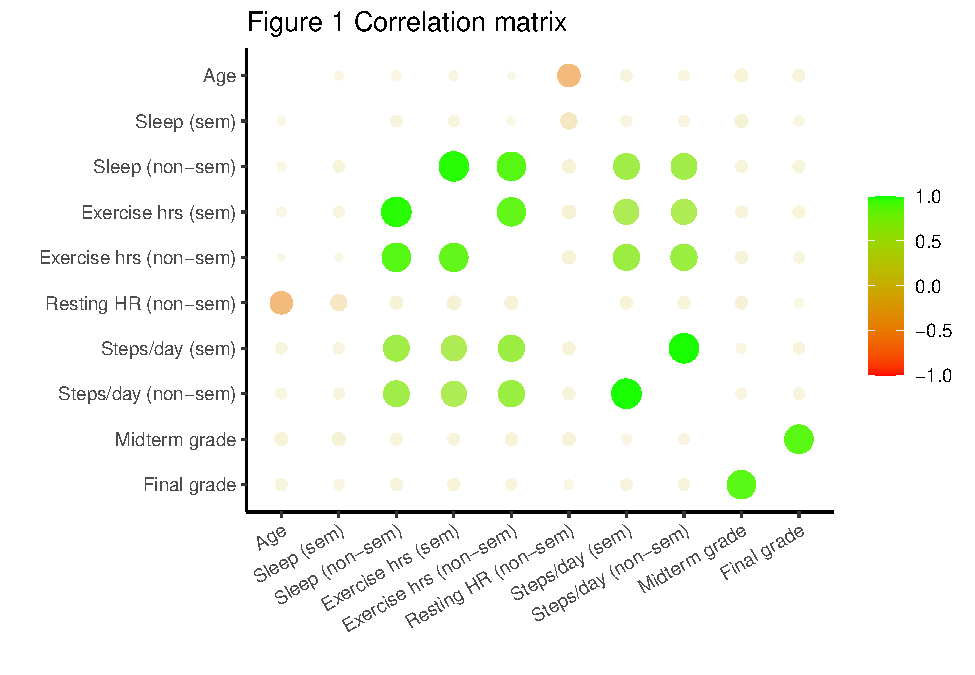
\includegraphics{assignment_2_files/figure-latex/pressure-1.pdf}

\begin{table}

\caption{\label{tab:unnamed-chunk-3}Correlation between variables in the study}
\centering
\fontsize{7}{9}\selectfont
\begin{tabular}[t]{l|l|>{\raggedright\arraybackslash}p{.44in}|>{\raggedright\arraybackslash}p{.44in}|>{\raggedright\arraybackslash}p{.44in}|>{\raggedright\arraybackslash}p{.44in}|>{\raggedright\arraybackslash}p{.44in}|>{\raggedright\arraybackslash}p{.44in}|>{\raggedright\arraybackslash}p{.44in}|>{\raggedright\arraybackslash}p{.44in}}
\hline
\textbf{term} & \textbf{Age} & \textbf{Sleep (sem)} & \textbf{Sleep (non-sem)} & \textbf{Exercise hrs (sem)} & \textbf{Exercise hrs (non-sem)} & \textbf{Resting HR (non-sem)} & \textbf{Steps/day (sem)} & \textbf{Steps/day (non-sem)} & \textbf{Midterm grade}\\
\hline
\cellcolor{gray!6}{Age} & \cellcolor{gray!6}{} & \cellcolor{gray!6}{} & \cellcolor{gray!6}{} & \cellcolor{gray!6}{} & \cellcolor{gray!6}{} & \cellcolor{gray!6}{} & \cellcolor{gray!6}{} & \cellcolor{gray!6}{} & \cellcolor{gray!6}{}\\
\hline
Sleep (sem) & -0.01 &  &  &  &  &  &  &  & \\
\hline
\cellcolor{gray!6}{Sleep (non-sem)} & \cellcolor{gray!6}{-0.01} & \cellcolor{gray!6}{0.04} & \cellcolor{gray!6}{} & \cellcolor{gray!6}{} & \cellcolor{gray!6}{} & \cellcolor{gray!6}{} & \cellcolor{gray!6}{} & \cellcolor{gray!6}{} & \cellcolor{gray!6}{}\\
\hline
Exercise hrs (sem) & -0.01 & 0.03 & 0.97 &  &  &  &  &  & \\
\hline
\cellcolor{gray!6}{Exercise hrs (non-sem)} & \cellcolor{gray!6}{0} & \cellcolor{gray!6}{0.01} & \cellcolor{gray!6}{0.9} & \cellcolor{gray!6}{0.87} & \cellcolor{gray!6}{} & \cellcolor{gray!6}{} & \cellcolor{gray!6}{} & \cellcolor{gray!6}{} & \cellcolor{gray!6}{}\\
\hline
Resting HR (non-sem) & -0.46 & -0.16 & 0.07 & 0.08 & 0.07 &  &  &  & \\
\hline
\cellcolor{gray!6}{Steps/day (sem)} & \cellcolor{gray!6}{0.04} & \cellcolor{gray!6}{-0.03} & \cellcolor{gray!6}{0.68} & \cellcolor{gray!6}{0.62} & \cellcolor{gray!6}{0.71} & \cellcolor{gray!6}{0.06} & \cellcolor{gray!6}{} & \cellcolor{gray!6}{} & \cellcolor{gray!6}{}\\
\hline
Steps/day (non-sem) & 0.03 & -0.03 & 0.68 & 0.62 & 0.71 & 0.05 & 0.99 &  & \\
\hline
\cellcolor{gray!6}{Midterm grade} & \cellcolor{gray!6}{0.07} & \cellcolor{gray!6}{0.07} & \cellcolor{gray!6}{0.05} & \cellcolor{gray!6}{0.05} & \cellcolor{gray!6}{0.06} & \cellcolor{gray!6}{-0.06} & \cellcolor{gray!6}{-0.02} & \cellcolor{gray!6}{-0.03} & \cellcolor{gray!6}{}\\
\hline
Final grade & 0.04 & 0.03 & 0.04 & 0.05 & 0.03 & 0.01 & -0.04 & -0.04 & 0.89\\
\hline
\end{tabular}
\end{table}

\hypertarget{question-3---relationship-between-university-program-and-resting-heart-rate}{%
\section{Question 3 - Relationship between University Program and
Resting heart
rate}\label{question-3---relationship-between-university-program-and-resting-heart-rate}}

\hypertarget{step-one---decide-on-most-appropriate-test}{%
\subsection{Step one - Decide on most appropriate
test}\label{step-one---decide-on-most-appropriate-test}}

To decide on the most appropriate statistical test, the data was first
assessed for normality. Graphical assessment of data in Figure 2 suggest
that there is some right-ward shift in the data. The QQ plot in Figure 3
also shows significant deviation from the QQ line. It is therefore not
necessary to conduct other tests, and the data should be considered
non-parametric. However since the sample size in all three groups is
larger than 30, the Central Limit Theorem applies and we can utilise
tests that usually rely on the data being normally distributed.

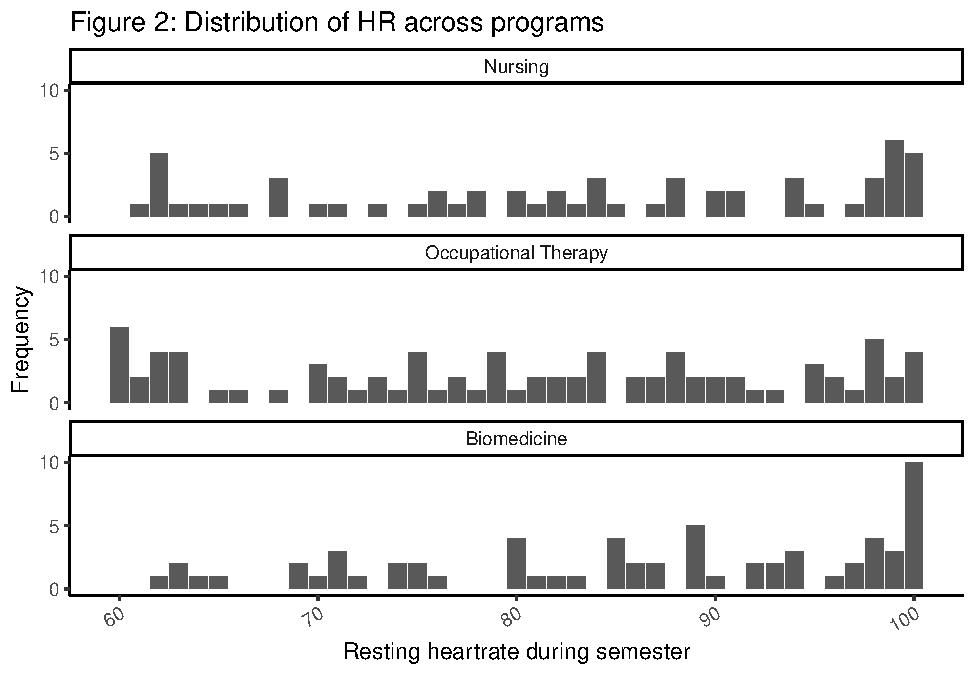
\includegraphics{assignment_2_files/figure-latex/distribution of results`-1.pdf}

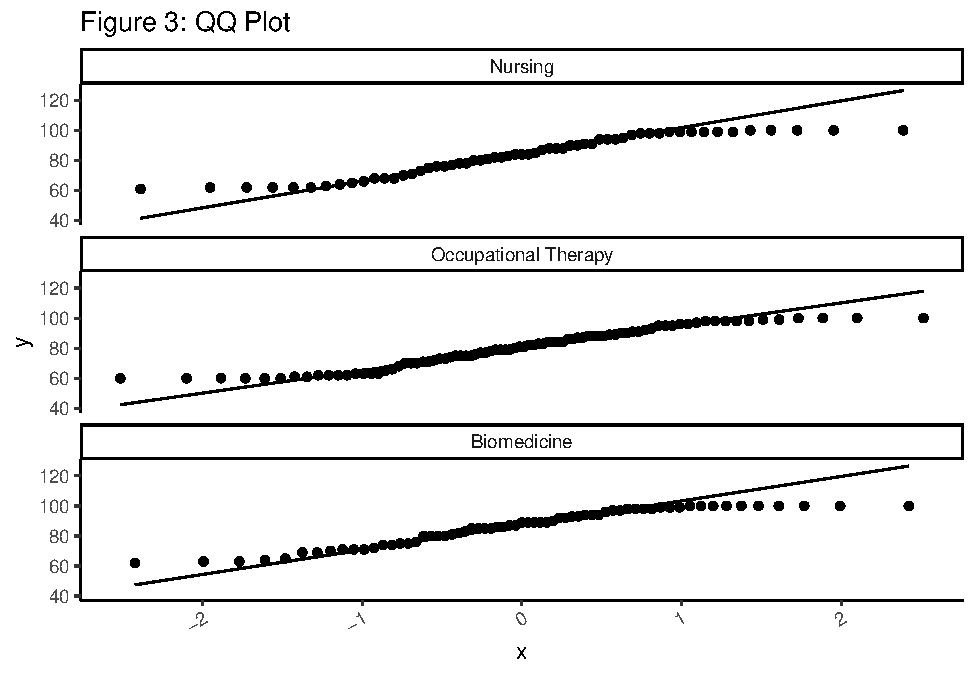
\includegraphics{assignment_2_files/figure-latex/qq plot-1.pdf}

Since we are comparing three different categories, a one way anova test
is the most appropriate test.

\hypertarget{state-hypothesis}{%
\subsection{State Hypothesis}\label{state-hypothesis}}

\(H_o\): There is no difference in the mean resting heart rate during
the semester among students in the three university programs

\(H_\alpha\): At least one university program has a different mean
resting heart rate during the semester.

\hypertarget{set-alpha}{%
\subsection{Set alpha}\label{set-alpha}}

The alpha chosen for this test is .05 as this is the most common in the
literature.

\hypertarget{calulcate-test-statistic}{%
\subsection{Calulcate test statistic}\label{calulcate-test-statistic}}

The results for the one-way anova are presented in Table 3. There is a
difference in the results between the resting heart-rate during the
semester for the students in the three programs, F = 4.03 and p = 0.02),
meaning that the probability that this result occurred by chance alone
was well below the .05 threshold chosen for this test. Since the value
of the one-way anova was significant, a pairwise-comparison with
Bonferroni adjustment was made in Table 4. Here we find that the
adjusted p-value for the comparison of means for Biomedical and
Occupational Therapy students was 0.02, suggesting that there is a
statistically significant difference between these two groups.

\begin{table}

\caption{\label{tab:unnamed-chunk-5}One-Way Anova of of heart rate during semester across programs}
\centering
\fontsize{7}{9}\selectfont
\begin{tabular}[t]{l|r|r|r|r|r}
\hline
\textbf{term} & \textbf{df} & \textbf{sumsq} & \textbf{meansq} & \textbf{statistic} & \textbf{p.value}\\
\hline
\cellcolor{gray!6}{Program} & \cellcolor{gray!6}{2} & \cellcolor{gray!6}{1289.86} & \cellcolor{gray!6}{644.93} & \cellcolor{gray!6}{4.03} & \cellcolor{gray!6}{0.02}\\
\hline
Residuals & 205 & 32792.33 & 159.96 & NA & NA\\
\hline
\end{tabular}
\end{table}

\begin{table}

\caption{\label{tab:unnamed-chunk-5}Pairwise comparison of heart rate during semester across programs with Bonferroni adjustment}
\centering
\fontsize{7}{9}\selectfont
\begin{tabular}[t]{l|r|l|r|r|r}
\hline
\textbf{First program} & \textbf{Mean} & \textbf{Second program} & \textbf{Mean } & \textbf{Difference between means} & \textbf{p.value}\\
\hline
\cellcolor{gray!6}{Occupational Therapy} & \cellcolor{gray!6}{80.26} & \cellcolor{gray!6}{Nursing} & \cellcolor{gray!6}{83.17} & \cellcolor{gray!6}{-2.91} & \cellcolor{gray!6}{0.53}\\
\hline
Biomedicine & 86.18 & Nursing & 83.17 & 3.02 & 0.56\\
\hline
\cellcolor{gray!6}{Biomedicine} & \cellcolor{gray!6}{86.18} & \cellcolor{gray!6}{Occupational Therapy} & \cellcolor{gray!6}{80.26} & \cellcolor{gray!6}{5.92} & \cellcolor{gray!6}{0.02}\\
\hline
\end{tabular}
\end{table}

\hypertarget{reject-or-retain-hypothesis}{%
\subsection{Reject or retain
hypothesis}\label{reject-or-retain-hypothesis}}

As a result of the analysis of this test above, we have rejected the
null hypothesis because there is a statistically significant difference
between the Resting heart rate during semester of Occupational Therapy
and Biomedical students.

\hypertarget{question-4---sleep-during-semester}{%
\section{Question 4 - Sleep during
semester}\label{question-4---sleep-during-semester}}

\hypertarget{decide-on-most-appropriate-test}{%
\subsection{Decide on most appropriate
test}\label{decide-on-most-appropriate-test}}

Comparing the heart rate of the same individuals both during and after
semester is an example of paired sample, and therefore a paired t-test
is the most appropriate analysis.

\hypertarget{state-hypothesis-1}{%
\subsection{State hypothesis}\label{state-hypothesis-1}}

\(H_o\): The average time spent sleeping by participants during the
semester is equal to the average time spent sleeping outside of the
semester.

\(H_\alpha\): The average time spent sleeping by participants during the
semester is not equal to the mean time spent sleeping outside of the
semester.

\hypertarget{set-alpha-1}{%
\subsection{Set alpha}\label{set-alpha-1}}

The alpha chosen for this test is .05 as this is the most common in the
literature.

\hypertarget{calulcate-test-statistic-1}{%
\subsection{Calulcate test statistic}\label{calulcate-test-statistic-1}}

Table 5 shows that the average time spent sleeping for students in
semester is 426 minutes, whereas the average time spent sleeping outside
of semester is 458. To test if this value is significant we consider the
results of a paired t-test in Table 6. The p-value for this test is .00
which suggests that the difference between the two means is
statistically significant.

\begin{table}

\caption{\label{tab:unnamed-chunk-7}Time spent sleeping during and outside semester}
\centering
\fontsize{7}{9}\selectfont
\begin{tabular}[t]{l|r|r|r}
\hline
\textbf{variable} & \textbf{Respondents} & \textbf{Mean} & \textbf{sd}\\
\hline
\cellcolor{gray!6}{Hours of sleep per day during semester (average)} & \cellcolor{gray!6}{250} & \cellcolor{gray!6}{426} & \cellcolor{gray!6}{45}\\
\hline
Hours of sleep per day outside semester (average) & 250 & 458 & 42\\
\hline
\end{tabular}
\end{table}

\begin{table}

\caption{\label{tab:unnamed-chunk-7}Results of paired t-test of Sleep during and outside of semester}
\centering
\fontsize{7}{9}\selectfont
\begin{tabular}[t]{r|r|r|r|r|r|l|l}
\hline
\textbf{Difference between means} & \textbf{t} & \textbf{p.value} & \textbf{parameter} & \textbf{conf.low} & \textbf{conf.high} & \textbf{method} & \textbf{alternative}\\
\hline
\cellcolor{gray!6}{-31.95} & \cellcolor{gray!6}{-8.38} & \cellcolor{gray!6}{0} & \cellcolor{gray!6}{249} & \cellcolor{gray!6}{-39.45} & \cellcolor{gray!6}{-24.44} & \cellcolor{gray!6}{Paired t-test} & \cellcolor{gray!6}{two.sided}\\
\hline
\end{tabular}
\end{table}

\hypertarget{reject-or-retain-hypothesis-1}{%
\subsection{Reject or retain
hypothesis}\label{reject-or-retain-hypothesis-1}}

Because the two means are different we reject null hypothesis that the
two means are the same

\hypertarget{question-5-university-satisfaction-and-unviersity-program}{%
\section{Question 5 University satisfaction and unviersity
program}\label{question-5-university-satisfaction-and-unviersity-program}}

\hypertarget{decide-on-most-appropriate-test-1}{%
\subsection{Decide on most appropriate
test}\label{decide-on-most-appropriate-test-1}}

Because we are comparing two categorical variables, the chi squared test
is the most appropriate way to check if these variables are related.

\hypertarget{state-hypothesis-2}{%
\subsection{State hypothesis}\label{state-hypothesis-2}}

\(H_o\): University satisfaction status is independent of the university
program.

\(H_\alpha\): University satisfaction status is dependent on the
university program.

\hypertarget{set-alpha-2}{%
\subsection{Set alpha}\label{set-alpha-2}}

The alpha chosen for this test is .05 as this is the most common in the
literature.

\hypertarget{calulcate-test-statistic-2}{%
\subsection{Calulcate test statistic}\label{calulcate-test-statistic-2}}

As shown in Table 7, a similar number of participants are completely
satisfied across all programs.

\begin{table}

\caption{\label{tab:unnamed-chunk-8}Share of participants completely satisfied across programs}
\centering
\fontsize{7}{9}\selectfont
\begin{tabular}[t]{l|r|r|r}
\hline
\textbf{Program} & \textbf{Participants} & \textbf{Share completely satisfied (\%)} & \textbf{sd}\\
\hline
\cellcolor{gray!6}{Nursing} & \cellcolor{gray!6}{59} & \cellcolor{gray!6}{56} & \cellcolor{gray!6}{0.5007300}\\
\hline
Occupational Therapy & 84 & 61 & 0.4913188\\
\hline
\cellcolor{gray!6}{Dentistry} & \cellcolor{gray!6}{42} & \cellcolor{gray!6}{57} & \cellcolor{gray!6}{0.5008703}\\
\hline
Biomedicine & 65 & 51 & 0.5038315\\
\hline
\end{tabular}
\end{table}

A chi-squared test was performed, and \(\chi 2\) is 1.49 and the p-value
is 0.68. There is therefore no evidence from these tests that the values
are significantly different.

\hypertarget{reject-or-retain-hypothesis-2}{%
\subsection{Reject or retain
hypothesis}\label{reject-or-retain-hypothesis-2}}

Given the p-value is less than .05, we fail to reject the null
hypothesis that satisfaction is independent of program.

\hypertarget{question-6}{%
\section{Question 6}\label{question-6}}

\hypertarget{decide-on-most-appropriate-test-2}{%
\subsection{Decide on most appropriate
test}\label{decide-on-most-appropriate-test-2}}

Given we are testing the effect of multiple variables on a continuous
outcome variable (Resting heart rate outside of semester) a linear
regression is the most appropriate test.

The equation for the regression is:

\[
\begin{split}
\operatorname{`Resting\ heart\ rate\ outside\ of\ semester\ (BPM)`} = \alpha +\\ \beta_{1}(\operatorname{Age}) +\\ \beta_{2}(\operatorname{`Steps\ per\ day\ during\ semester\ (average)`}) +\\ \beta_{3}(\operatorname{`Exercise\ during\ semsester\ (minutes\ per\ week)`}) +\\ \beta_{4}(\operatorname{`Final\ grade\ (\%)`}) +\\ \epsilon
\end{split}
\]

\hypertarget{state-hypothesis-3}{%
\subsection{State hypothesis}\label{state-hypothesis-3}}

\(H_o\): Resting heart rate outside of semester is not correlated with
age, steps per day during semester, exercise during semester or final
grade

\(H_\alpha\): Resting heart rate outside of semester is correlated with
any of age, steps per day during semester, exercise during semester or
final grade

\hypertarget{set-alpha-3}{%
\subsection{Set alpha}\label{set-alpha-3}}

The alpha chosen for this test is .05 as this is the most common in the
literature.

\hypertarget{calulcate-test-statistic-3}{%
\subsection{Calulcate test statistic}\label{calulcate-test-statistic-3}}

The results in Table 8 show that after controlling for exercise, steps
per day, and final grade, resting heart rate in this population is 1.8
beats per minute lower for every year of extra age. The p-value for this
estimate is less than .001, suggesting a statistically significant
relationship. For all other variables p is greater than .05 and there is
therefore no evidence of a relationship.

\begin{table}

\begin{threeparttable}
\caption{\label{tab:unnamed-chunk-11}Results of linear regression against resting hear-rate outside of semester}
\centering
\fontsize{7}{9}\selectfont
\begin{tabular}[t]{l|c|c|c}
\hline
\textbf{\textbf{Characteristic}} & \textbf{\textbf{Beta}} & \textbf{\textbf{95\% CI}} & \textbf{\textbf{p-value}}\\
\hline
\cellcolor{gray!6}{Age} & \cellcolor{gray!6}{-1.8} & \cellcolor{gray!6}{-2.2, -1.3} & \cellcolor{gray!6}{<0.001}\\
\hline
Steps per day during semester (average) & 0.00 & 0.00, 0.00 & 0.5\\
\hline
\cellcolor{gray!6}{Exercise during semsester (minutes per week)} & \cellcolor{gray!6}{0.01} & \cellcolor{gray!6}{-0.04, 0.07} & \cellcolor{gray!6}{0.6}\\
\hline
Final grade (\%) & 0.06 & -0.14, 0.26 & 0.6\\
\hline
\multicolumn{4}{l}{\rule{0pt}{1em}\textsuperscript{1} CI = Confidence Interval}\\
\end{tabular}
\begin{tablenotes}
\small
\item [] R² = 0.219; Adjusted R² = 0.207; Sigma = 11.1; Statistic = 17.2; p-value = <0.001; df = 4; Log-likelihood = -954; AIC = 1,920; BIC = 1,941; Deviance = 30,183; Residual df = 245; No. Obs. = 250
\end{tablenotes}
\end{threeparttable}
\end{table}

This model underwent several robustness tests and their results in
Figure 4. In the first plot that the residuals are evenly spread above
and below the fitted line, suggesting normality. In the second (Normal
Q-Q) plot the residuals form a straight line without much deviation, and
the third plot shows even spread across the fitted line - suggesting
minimal heteroskedasticity. In the final graph there are few outliers
that have significant residuals on the model. While not perfect outputs,
these four tests suggest high robustness of the model.

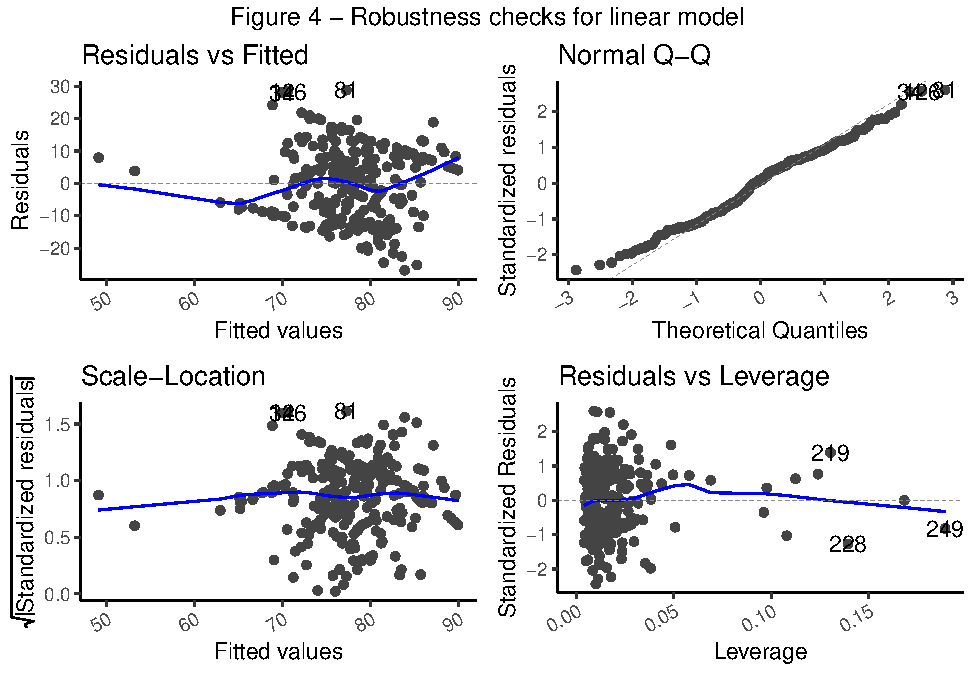
\includegraphics{assignment_2_files/figure-latex/unnamed-chunk-12-1.pdf}

\hypertarget{reject-or-retain-hypothesis-3}{%
\subsection{Reject or retain
hypothesis}\label{reject-or-retain-hypothesis-3}}

Since there is a statistically significant relationship between age and
heart-rate, we reject the null-hypothesis.


\end{document}
